\section{Sprint}
Eine kleine Gruppe Studenten wollte anhand einer Produkt-Idee das Prinzip des Sprints durchlaufen, da dieser Prozess sehr gefragt scheint. Bei dieser Idee handelt es sich um eine Online-Plattform für die Agrarbranche, wobei das Team noch ganz am Anfang der Konzeptfindung und Entwicklung steht. Diesbezüglich sollte der Sprint erste Ergebnisse liefern, ob die Idee beim Endkunden angenommen wird oder nicht. Allerdings stellte sich heraus, dass der Prozess, wie vorgegeben, für diesen Zweck nicht genau so umsetzbar ist. Der Ablauf der Sprints, sowie Abwandlungen sind im Folgenden genauer erläutert.
\subsection*{Tag 1}
\paragraph{Long Term Goal}
Der erste Tag startet mit einer sehr ertragreichen Gruppendiskussion zum Thema Projekt-Vision. Es wird schnell klar, dass bereits an dieser Stelle die Ansichten der einzelnen Team-Mitglieder teilweise stark voneinander abweichen. Nichtsdestotrotz ist es der Gruppe doch möglich, sich aufeinander abzustimmen und ein Long Term Goal aufzustellen, mit dem jeder Teilnehmer einverstanden ist.
%Gruppendiskussion
%Wo sehen wir uns in 6 Monaten? in 1 Jahr? in 5 Jahren?
%Warum wird das Projekt durchgeführt?
%
%Ziele:
%1/2 Jahr: Testbarer Prototyp
%1 Jahr: Beta-Version
%3 Jahre: Erweiterungen (Funktionalität, Branchen, Gebiete)
%Stichwortsammlung
%
%Resultat: Digitale und effiziente Plattform zur Ressourcenauslastung
\paragraph{Sprint-Fragen}
Weniger überraschend ist die Anzahl der Sprint-Fragen, die vom Team gestellt wurden. Besonders vor einer großen Aufgabe, wie dieser, treten viele Bedenken und Befürchtungen auf, welche im Rahmen dieser Aufgabe sehr schnell gesammelt werden können. Damit wird auch schnell klar, welche unterschiedlichen Teilbereiche das Gesamtprojekt zusätzlich anschneidet und in welchen Gebieten besondere Vorsicht geboten ist. Für das Team ist es in diesem Fall auch hilfreich zu verstehen, welche Risiken die einzelnen Teilnehmer sehen. An diesem Beispiel ist gut zu erkennen, dass es besonders zu Beginn eines solchen Projektes sehr viele offene Fragen gibt, von denen die Mehrzahl sicher nicht im Sprint behandelbar ist. Trotzdem fühlt es sich für das Team im Allgemeinen gut an, diese Bedenken an der Stelle festzuhalten und auch über den Workshop hinaus im Hinterkopf zu behalten. So entstehen beim Team AgriShare 16 Sprint-Fragen.

%Sammeln aller Fragen des Teams bezüglich des Projekts
%Risiken, Ängste...
%Annahmen und potentielle Hürden in Fragen umformulieren
%Die meisten Fragen sind vermutlich nicht im Sprint behandelbar, aber werden im Hinterkopf behalten.
%
%Resultat: 
%
%\begin{enumerate}
%	\item Wie ermöglicht man eine einfache Nutzung für ältere Personen?
%	\item Wie schaffe ich es, komplexe Vorgänge in einfache Schritte aufzubrechen?
%	\item Wie kriegen wir Kunden?
%	\item Wie kriegen wir loyale Beta-Tester?
%	\item Wie kann ich die Wetter-Daten sinnvoll einbauen?
%	\item Wie kann ich die Anwendung als komplette Service-Plattform auslegen?
%	\item Wie müssen wir das Design gestalten, um unsere Zielgruppe anzusprechen?
%	\item Wie können wir den rechtlichen Rahmen einhalten?
%	\item Wie verdienen wir Geld dabei?
%	\item Wie stellen wir sicher, dass alle benötigten Funktionalitäten abgedeckt sind?
%	\item Was macht uns besser als die Konkurrenz?
%	\item Wo sind die Hotspots?
%	\item Wie können wir unsere Corporate Identity auf die Zielgruppe abstimmen?
%	\item Wie bringen wir genug Startkapital auf? (mit/ohne Investoren)
%	\item Welche Kosten kommen auf uns zu?
%	\item Wie kann eine Vermittlung mit Verischerung durchgeführt werden?
%\end{enumerate}
\paragraph{Map}
In diesem Team ist die Erstellung der Map keine einfache Aufgabe, wie sich früh herausstellt. In vielen Bereichen des Projekts wird klar, dass die Teilnehmer sehr unterschiedliche Ansichten haben. Daher entstehen zahlreiche Diskussionen sowohl über die Struktur der Plattform, als auch Begriffsklärungen. Im Rahmen der Kundengruppen wird das Konzept eines Premium-Nutzers aufgeworfen. Nach einigen Diskussionen wird diese Idee allerdings zunächst verworfen, aber im Hinterkopf behalten. Bei den Begriffsklärungen fällt besonders auf, dass die Kundensicht und die technische Umsetzung weit auseinander driftet. Da die Benutzung für den Endnutzer möglichst intuitiv und einfach sein soll, müssen die einzelnen Kompnenten klar definiert sein. Darüber ist sich das Team auch einig, allerdings ist dies leichter gesagt als getan. Unerwarteterweise wirft genau das großen Diskussionsbedarf auf und Abstimmung untereinander ist zwingend nötig. Obwohl diese Aufgabe sehr anstrengend ist, zeigt sich der Mehrwert darauf am Ende ganz klar. Jeder Teilnehmer hatte vor dem Sprint eine andere Grundperspektive davon, was letztlich im Produkt enthalten sein soll. Schließlich ist es der Gruppe gelungen, diese Ansichten miteinander zu vereinen und mit der Map ein gutes Fundament zu legen. Letztendlich ist es gelungen, das anfangs sehr kompliziert scheinende Projekt auf zwölf einzelne Schritte herunterzubrechen. Außerdem gibt es während der Übung einen überraschenden Nebeneffekt. Durch die vielen Diskussionen über einzelne Komponenten und deren technische Darstellung wird nebenbei auch ein Klassendiagramm erstellt, was dem Team zusätzliche Arbeit in der Zukunft erspart.


%Einfach
%Kundenorientiert
%
%Potential von Premium-Nutzern aufgekommen - wurde verworfen
%Sehr lange Diskussionen und aneinander Vorbeireden
%Unklarheit der Aufgabenstellung zu Beginn
%Diskussion über Details, von denen jeder andere Ansichten hatte
%Klassendiagramm konnte parallel dazu erstellt werden!
%Eindeutige Begriffsbildungen!
%
%Aufsbrechen des Gesamtprojekts in Einzelschritte
%Gruppendiskussionen
%Begriffsklärung sehr wichtig
%\begin{figure}[h!]
%	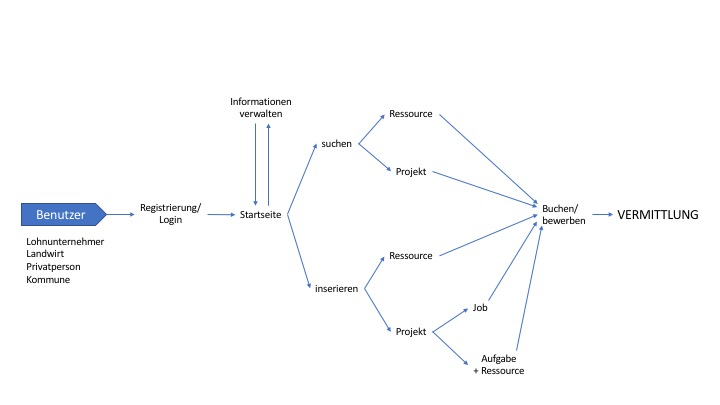
\includegraphics[width=\textwidth]{99_IMG/03_Sprint/map}
%	\caption{Projekt Map}
%	\label{fig:map}
%\end{figure}
%
%Wie in \ref{fig:map} dargestellt ist, wurden die Benutzer nochmal in Einzelgruppen eingeteilt. Das diente dem besseren Verständis im Team. Diese Benutzer müssen sich zuerst authentifizieren durch Login oder Registrierung. Danach sollen sie auf die Startseite geleitet werden, von wo aus sie verschiedene Möglichkeiten haben sollen. Die Nutzer können dann ihre Informationen verwalten, nach Inseraten suchen oder selber inserieren. Bei der Suche wird nur zwischen Ressourcen oder Projekten unterschieden, wohingegen ein Inserat ebenfalls eine Ressource oder ein Projekt beinhalten kann, dieses aber nochmal in Job oder Aufgabe unterteilt ist. Eine Aufgabe ist so definiert, dass es auch Ressourcen beinhalten kann. Nach diesen Abläufen kommt es typischerweise zu einer Buchung oder Bewerbung. Nach der Bestätigung wurde also eine Vermittlung durchgeführt, was das Ende des Prozesses beschreibt.

\paragraph{Ask the Experts}
Die Expertenrunden laufen in diesem Team zunächst wie geplant ab. Die meisten Fachleute kommen hier tatsächlich aus dem Sprint-Team selbst. So wird über die Bereiche Rechnungswesen und -stellung, typische Fehlerquellen und den aktuellen Vermittlungsvorgang vorgetragen. Da diese Themen ohnehin schon im Rahmen früherer Meetings besprochen worden sind, ergeben sich auch wenig neue Einsichten. Obwohl diese Aufgabe dazu gedacht ist, bereits Gehörtes erneut zu wiederholen und bei Unklarheiten Fragen zu stellen, ist der Mehrwert daraus nicht ganz klar. Erst als der letzte Experte dazustößt, welcher ein potentieller Endkunde sein könnte, werden neue Einsichten gewonnen. Als klarer Vertreter der Kundenseite, deutet dieser auf Unklarheiten bezüglich des Gesamtprojektes hin. Aufgrund der vielen wertvollen Informationen von diesem Experten wird das Gespräch nicht nach 30 Minuten abgebrochen, wie vorgegeben. Daher werden die restlichen geplanten Punkte für den ersten Tag bereits auf Tag zwei verschoben. Das Projektteam ist sich bei dieser Prozessabwandlung einig, da das Gespräch mit diesem Experten jedem dabei hilft, den Kunden besser zu verstehen und das Projekt darauf zu beschränken, was der Kunde tatsächlich braucht.

Während aller Expertenrunden schreibt das restliche Team Notizen auf Klebezettel und legt diese beiseite. Am Ende werden alle Notizen gesammelt und an einem Whiteboard angebracht. Die geplanten weiteren Punkte werden, wie bereits erwähnt, auf Tag 2 verschoben.
%
%Experten:
%Theresa Jakob: Rechnungswesen
%Matthias Coufal, Verena Schmöller: Ablauf der Buchung über Maschinenring
%Sebastian Brunthaler: Typische Fehlerquellen in Projektteams
%Landwirt: allgemeiner Eindruck des Projektes, Unklarheiten?
%Masterand Horsch: Kundensicht
%
%Rechnungswesen: 
%Erhalten der Originalrechnung: Wenn per Post verschickt, Papierform ist Originalrechnung. Wenn per E-Mail verschickt, elektronische Form ist Originalrechnung (nicht der Ausdruck). 
%
%Fehlerquellen:
%Verschieben der Aufgaben von Person zu Person. Keine Verantwortung für eigene Aufgaben übernehmen.
%
%Prozess MR:
%Vermittlung der Maschinen/Dienstleistungen telefonisch. Meist nicht über MR, da sich Landwirte meist untereinander kennen. Abrechnung immer über MR, da der bürokratische Aufwand der Rechnungsstellung und Dieselbeihilfe abgenommen wird. Preis: Vorschläge von MR (Preiskatalog), aber individuell einstellbar.
%
%Kundensicht: Möglichkeit, Maschinen mit Versicherung zu vermieten. Lohnunternehmer-Prozess bisher, allerdings mehr Potential in Privatpersonen, da sehr große Zielgruppe. Fokus auf kleineren Hausarbeiten
%
%Da ein sehr hilfreicher potentieller Endkunde ebenfalls als Experte eingeladen wurde, welcher sehr viele Einsichten über potentielle Unklarheiten geben konnte, wurde der geplante Ablauf des Sprints bereits am Tag 1 abgewandelt. Es wurde der Fokus darauf gelegt, so viel wie möglich mit diesem Experten zu besprechen und die weiteren Punkte auf den nöchsten Tag zu legen.

\paragraph{Logo und Name}
Parallel zum eigentlichen Sprint-Prozess ist das Team an Tag 1 so motiviert, dass in den Pausen kleinere Diskussionen bezüglich Logo und Name des Produkts entstehen. Das führt dazu, dass im Anschluss an den offiziellen Sprint das finale Logo und auch der letztendliche Produktname entstehen.

\paragraph{Fazit}
Nach dem ersten Tag ist das Gesamtfeedback des Teams sehr positiv. Der Prozess wird bisher als sehr hilfreich angesehen, obwohl die Erwartungen im Vorfeld sehr niedrig waren. Unter Anderem war es möglich in nur einem Tag potentielle Risiken im Vorfeld zu eliminieren. Außerdem wird vermutet, dass die Entwicklung allgemein erleichtert wird, da viele Unklarheiten, welche sonst in der Implementierung Probleme machen würden, bereits beseitigt wurden. Da das ganze Team fokussiert und konzentriert mitarbeitete, war der gesamte Tag äußerst produktiv. So entstanden auch viele Ideen bezüglich möglicher Erweiterungen und weiterer Anwendungsgebiete. Auch vorher verworfene Anwendungsgebiete wurden wieder aufgerollt und ins Gedächtnis gerufen. Des Weiteren sind sehr viele Bedenken des Teams schriftlich festgehalten, was das Team durchaus positiv stimmt. Im Allgemeinen entstanden sehr ertragreiche Diskussionen und Ideenfindungen. Es war auch sehr wichtig, die Erwartungen aller Teammitglieder aufeinander abzustimmen und sicherzugehen, dass alle die gleichen Ansichten haben. Dabei geht es nicht nur um zeitliche Erwartungen, sondern auch was das Projekt beinhaltet und was tatsächlich das Produkt darstellen soll. Denn jedes Teammitglied hatte für sich selbst ein sehr klares Bild von dem Projekt. Diese Ansichten waren allerdings von Person zu Person sehr unterschiedlich. Daher war Tag 1 vor allem auch im Bereich 'Teambuilding' sehr erfolgreich.

Obwohl die Expertenrunden zunächst nicht sehr hilfreich schienen, zeigt sich der Mehrwert davon dennoch. So sind die Notizen, welche während dieser Aufgabe entstanden, essentiell für den weiteren Verlauf des Projekts. Die Themen wurden zwar schon des Öfteren besprochen, jedoch nie schriftlich festgehalten. Daher war es durchaus sinnvoll, diese Dinge aufzuschreiben, um zu garantieren, dass sie nicht in Vergessenheit geraten, wenn nicht mehr darüber diskutiert wird.

\subsection*{Tag 2}
\paragraph{Notizen sortieren und bewerten}
Da am Tag 1 nicht alle geplanten Aufgaben abgearbeitet werden können, müssen die letzten drei Punkte am nächsten Tag behandelt werden. Diese nehmen allerdings nicht viel Zeit in Anspruch, sodass das Team schnell wieder in den eigentlichen Aublauf einsteigen kann. Das Sortieren und Bewerten der Notizen läuft ohne viele Diskussionen ab, da sich die Teilnehmer meist einig sind. So werden am Ende zwei Haftnotizen mit den meisten Stickern an der Map angebracht.

%Zuerst werden die gesammelten Notizen sortiert. Dabei sortiert das gesamte Team zuerst Duplikate aus und teilt die restlichen Zettel in inhaltlich logische Gruppen ein. Für diese Gruppen wurden zusätzlich noch Überbegriffe festgelegt und ebenfalls an dem Whiteboard angebracht. Anschließend wurden Sticker verteilt - zwei Sticker pro Person und 4 für den Decider. Jedes Teammitglied sollte sich nun das Long Term Goal, sowie die Sprint-Fragen erneut vor Augen führen. Danach werden die Sticker in einer stillen Abstimmung an die Notizen angebracht, die für den Sprint-Zeitraum als am Wichtigsten erachtet werden. Diese Notizen wurden dann an dem Whiteboard mit der Map angebracht, passend zu den jeweiligen Schritten.

\paragraph{Fokus des Sprints}
Nun ist es die Aufgabe des Deciders, den Fokus für diesen Sprint einzugrenzen. Da das Projekt zu diesem Zeitpunkt noch am Anfang der Entwicklung steht, müssen für einen sinnvollen und testbaren Prototypen fast alle Bereiche der Map abgedeckt werden. Deshalb wird der Fokus auf die gesamte Map gerichtet, was in der Spezifikation nicht so vorgesehen ist. Jedoch hat der Decider entschieden, dass nur eine teilweise Prototypisierung des Projekts zu einseitige Ergebnisse hervorrufen würde und deshalb nicht sinnvoll ist.

\paragraph{Lighting Demos}
%Liste mit für das Projekt interessante Produkte
%
%Liste:
%\begin{itemize}
%	\item Airbnb
%	\item Google Maps
%	\item Uber
%	\item Tractorpool
%	\item ...
%\end{itemize}
Jedes Teammitglied beschäftigt sich mit 2-3 Produkten und hebt für das Projekt relevante Teile hervor. Die Übung wird allgemein als eine sehr gute Inspiration erachtet und es gibt nur sehr wenige Diskussionen. 
Bei dieser Aufgabe fällt auf, dass zwar die meisten Produkte schon im Vorhinein bekannt waren, sich allerdings die Meinungen darüber im Team selbst sehr unterscheiden.

%App reiner Assistent (nicht volle Funktionalität)
\paragraph{Aufgabenverteilung}
Die Aufgabenverteilung erfolgt reibungslos, da sich das Team sehr schnell darauf einigen kann, wer welche Bereiche bearbeiten soll. Da der Fokus in diesem Fall sehr breit gefächert ist, werden jeder Person jeweils 3 Schritte zugeteilt.

\paragraph{Sketch}
Bereits nach den ersten 30 Minuten der Ideensammlung fällt auf, dass der Prozess so nicht hilfreich für das Projekt ist. Es werden zu viele Screens für den Prototypen benötigt, welche unmöglich innerhalb der kurzen Zeit von wenigen Personen erstellt werden können. Außerdem ist es besonders wichtig, dass die Screens eine einheitliche Maske und einen ähnlichen Aufbau haben. Deshalb ist es nicht sinnvoll, jede Person ein eigenes Set an Bildschirmen bauen zu lassen. Nachdem also jeder eigene Ideen gesammelt hat, wird begonnen, die einzelnen Seiten mit der gesamten Gruppe groß auf einem Whiteboard zu erstellen. Hier fällt auf, dass es immer noch sehr viele Unklarheiten bezüglich der grundlegenden Funktionsweise gibt. Das Team führt sich allerdings immer wieder vor Augen, dass das Endprodukt nicht besonders ausgeflippt oder kreativ gestaltet sein muss, sondern einfach zu verstehen und nach einem einheitlichen Prinzip aufgebaut sein muss. Innerhalb des Nachmittags von Tag 2 schafft es das Team, eine einheitliche Maske zu erstellen und es kann die Startseite, sowie teilweise die Kartenansicht erstellt werden.
Zugunsten des Gesamtteams und des Projekterfolges wird am Ende von Tag 2 beschlossen, die Screens nach einem eigenen Prozess in Gruppenarbeit zu erstellen, anstatt dem Sprint-Prozess zu folgen.

\paragraph{Fazit}
Am Ende von Tag 2 ist das Team wiederum einer Meinung, was den Gesamtprozess angeht. Der Sketch-Prozess, wie spezifiziert, ist nicht sinnvoll für ein einheitliches Produkt mit vielen Screens. Das heißt nicht, dass die Herangehensweise grundsätzlich als falsch angesehen wird. Für kleinere Add-Ons, Zusatzfunktionen oder Design-Fragen könnte dies durchaus einen großen Mehrwert gegenüber "unserer" Herangehensweise haben. Nichtsdestotrotz war das Projektteam trotzdem sehr kreativ und fokussiert bei der Sache. Auch die Meinung von Nicht-Teammitgliedern ist durchaus wertvoll, was durch verschiedene Besucher zum Ausdruck kommt. Auch die Befürchtung, man könnte sich an unnötigen Details aufhängen, kann nicht bestätigt weden, da dies immer sehr gut eliminiert werden konnte. Da zu diesem Zeitpunkt bereits der komplette Sprint-Prozess abgewandelt wurde, sind die Rollen auch ineinander verschmolzen.

\subsection*{Tag 3}
Der Tag wird so begonnen, wie der Tag zuvor beendet wurde. Erstellen der verschiedenen Screens des Endproduktes mit dem gesamten Team. Um Zeit einzusparen, erstellt ein Teammitglied parallel dazu den digitalen Prototypen der erstellten Bildschirme. Obwohl der Tag wenig abwechslungsreich ist und sehr eintönig scheint, ist das Team dennoch sehr fokussiert und produktiv. Es entstehen wiederum zahlreiche Diskussionen, wobei man sich aber auf essentielle Dinge beschränkt.

\subsection*{Tag 4}
Bereits zu Beginn von Tag 4 wird klar, dass es wenig Sinn macht, den Prototypen so zu testen, da dieser noch zu wenig Inhalt hat. Deshalb wird beschlossen, dass die geplanten Tests verschoben werden und direkt nach dem Sprint damit begonnen wird, das Produkt ansatzweise zu implementieren. Ein weiterer Grund dafür, die Tests abzusagen, war, dass ein Usertest mit unserer Zielgruppe zu viel Aufwand für einen Tag wäre. Denn Landwirte sind vor allem im Sommer sehr beschäftigt und können nicht für 30 Minuten in die Stadt fahren. Deshalb wird beschlossen, zu einem späteren Zeitpunkt potentielle Tester zu besuchen und dort zu testen. Das Team führt die Erstellung der einzelnen Bildschirme fort, wie bereits an Tag 3.

\subsection*{Tag 5}
Am letzten Tag sind immer noch nicht alle Screens fertig skizziert, aber die Energie des Teams ist mittlerweile sehr niedrig. Deshalb wird die restliche Zeit genutzt, um nochmal alle Details zu klären, die restlichen Screens zu erstellen und sich auf ein Logo und einen Namen zu einigen. Dieses Ziel wird erreicht und das Team schließt den Sprint mit einem sehr guten Gefühl ab.

%\subsection*{Allgemeines Fazit - Sprint}

\subsection*{Evaluierung des Prozesses}
Wie bereits oben angedeutet, hatte das Projektteam allgemein sehr niedrige Erwartungen an den Prozess. Es wurde kein großer Mehrwert erwartet, weshalb am Ende jeder positiv überrascht von dem Ergebnis war. Hauptsächlich die ersten beiden Tage haben dem Team vermutlich sehr viel Arbeit und zukünftige Diskussionen erspart. Sehr positiv anzumerken ist, dass jeder Beteiligte sehr konzentriert mitgearbeitet hat und mit großem Arbeitswillen bei der Sache war. Das führte dazu, dass das Team während der ganzen 5 Tage in einem Flow war und dementsprechend sehr gute Arbeit und konstruktive Beiträge geleistet hat. Allerdings ist auch aufgefallen, dass der Prozess, wie vorgesehen, nicht sinnvoll für ein komplett neues Produkt ist. Dies beinhaltet zu viele Einzelteile und zu viele Details, die das ganze Team zusammen abklären muss. Durchaus sinnvoll wäre das für eine Erweiterung eines bestehenden Produktes. In der abgewandelten Variante dieses Teams wurden trotzdem viel mehr Ergebnisse erzielt als erwartet. In nur fünf Tagen konnte ein Konzept erstellt werden, alle Screens des Produktes gezeichnet werden und sich auf ein Logo und einen Brand-Name geeinigt werden. Da alle Teammitglieder hauptberuflich andere Dinge machen, wie ein Studium oder Vollzeitarbeit, hätte es ohne den Sprint wohl sehr lange gedauert, bis diese Dinge geklärt worden wären.

Diesbezüglich war sich das Team auch einig, einen Follow-Up Sprint zu starten, sobald das Grundprodukt implementiert ist und erste User-Tests gemacht wurden.
